\section{Überschrift Ebene eins}

Lorem ipsum dolor sit amet, consetetur sadipscing elitr, sed diam nonumy eirmod tempor invidunt ut labore et dolore magna aliquyam erat, sed diam voluptua. At vero eos et accusam et justo duo dolores et ea rebum. Stet clita kasd gubergren, no sea takimata sanctus est Lorem ipsum dolor sit amet. Lorem ipsum dolor sit amet, consetetur sadipscing elitr, sed diam nonumy eirmod tempor invidunt ut labore et dolore magna aliquyam erat, sed diam voluptua. At vero eos et accusam et justo duo dolores et ea rebum. Stet clita kasd gubergren, no sea takimata sanctus est Lorem ipsum dolor sit amet.

Zitat aus \cite{scheme} und \cite[17]{knuth}. Lorem ipsum dolor sit amet, consetetur sadipscing elitr, sed diam nonumy eirmod tempor invidunt ut labore et dolore magna aliquyam erat, sed diam voluptua. At vero eos et accusam et justo duo dolores et ea rebum.
Es folgt eine Abbildungen. Abbildung \ref{abb_einstein} kann referenziert werden.

\begin{figure}[htbp]
\centering
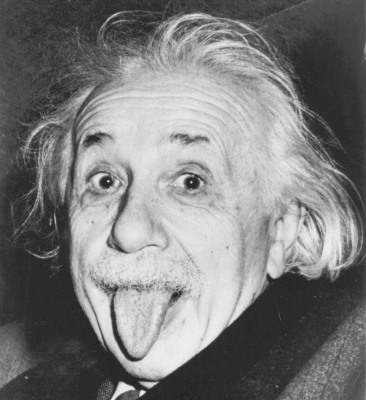
\includegraphics[scale=0.5]{einstein}
\caption{Beschreibung der Abbildung.}
\label{abb_einstein}
\end{figure}

\subsection{Überschrift Ebene zwei}

At vero eos et accusam et justo duo dolores et ea rebum. Stet clita kasd gubergren, no sea takimata sanctus est Lorem ipsum dolor sit amet. Lorem ipsum dolor sit amet, consetetur sadipscing elitr, sed diam nonumy eirmod tempor invidunt ut labore et dolore magna aliquyam erat, sed diam voluptua. At vero eos et accusam et justo duo dolores et ea rebum. Stet clita kasd gubergren, no sea takimata sanctus est Lorem ipsum dolor sit amet. Lorem ipsum dolor sit amet, consetetur sadipscing elitr, sed diam nonumy eirmod tempor invidunt ut labore et dolore magna aliquyam erat, sed diam voluptua.

\section{Aufzählungen, Tabellen und Programmcode}

Eine Aufzählung:

\begin{itemize}
\item Lorem ipsum
\item dolor sit amet
\item consetetur sadipscing elitr
\item sed diam nonumy
\end{itemize}
Eine nummerierte Aufzählung:

\begin{enumerate}
\item Erster Punkt
\item Zweiter Punkt
\item Dritter Punkt
\end{enumerate}
Es folgt Tabelle \ref{beispieltabelle}.

\begin{table}[htbp]
\centering
\begin{tabular}{lrc}
\toprule
Linksbündig & Rechtsbündig & Zentriert \\
\midrule
Lorem &  13 & amet \\ \addlinespace
ipsum & 104 & consetetur \\ \addlinespace
dolor &   7 & sadipscing \\ \addlinespace
sit   &  -5 & elitr \\
\bottomrule
\end{tabular}
\caption{Beschreibung der Tabelle.}
\label{beispieltabelle}
\end{table}

Programmcode im Fließtext: \lstinline{printf("Hello, world!\n");}.
Lorem ipsum dolor sit amet, consetetur sadipscing elitr, sed diam nonumy eirmod tempor invidunt ut labore et dolore magna aliquyam erat, sed diam voluptua. At vero eos et accusam et justo duo dolores et ea rebum. Stet clita kasd gubergren, no sea takimata sanctus est Lorem ipsum dolor sit amet.
Es folgt Programmlisting \ref{beispiellisting}.

\begin{lstlisting}[caption={Beschreibung des Listings.}, label=beispiellisting, frame=tblr, numbers=left]
#include <stdio.h>

int main(void)
{
    printf("Hello, world!\n");
}
\end{lstlisting}
Ein Listing ohne Titel, welches nicht im Listingverzeichnis aufgefühert wird:

\begin{lstlisting}
#include <stdio.h>

int main(void)
{
    printf("Hello, world\n");
}
\end{lstlisting}

Text kann \emph{kursiv} oder \textbf{fett} gesetzt werden.
Lorem ipsum dolor sit amet, consetetur sadipscing elitr, sed diam nonumy eirmod tempor invidunt ut labore et dolore magna aliquyam erat, sed diam voluptua. At vero eos et accusam et justo duo dolores et ea rebum. Stet clita kasd gubergren, no sea takimata sanctus est Lorem ipsum dolor sit amet. Lorem ipsum dolor sit amet, consetetur sadipscing elitr, sed diam nonumy eirmod tempor invidunt ut labore et dolore magna aliquyam erat, sed diam voluptua. At vero eos et accusam et justo duo dolores et ea rebum. Stet clita kasd gubergren, no sea takimata sanctus est Lorem ipsum dolor sit amet.
